\documentclass{jpconf}

\usepackage{amsmath}
\usepackage{citesort}
\usepackage[utf8]{inputenc}
\usepackage{graphicx}
\usepackage{float}
\usepackage{caption}
\usepackage{tikz}
\usepackage{wrapfig}
\usepackage{fancyhdr}
\usepackage{textcomp}

\usepackage{pgfplots}
\pgfplotsset{width=7cm,compat=1.8}

\pagestyle{fancy}

\lhead{\thepage}
\chead{}
\rhead{\bfseries Cosmic Calibration}
\lfoot{}
\cfoot{}
\rfoot{}


\newcommand{\curlH}{\mathcal{H}}
\newcommand{\gws}{\tilde{h}}




\bibliographystyle{unsrt}

\graphicspath{{images/}}








\begin{document}


\title{Cosmic Calibration of Gravitational Wave Detectors}




\author{Liam Wright}

\ead{1002990w@student.gla.ac.uk}
\address{University of Glasgow, Glasgow, G12 8QQ, United Kingdom}
 
\begin{abstract}
  With the second generation of ground-based gravitational wave detectors on the verge of being switched on, and a predicted detection rate of between $0.4 yr^{-1}$ and $400 yr^{-1}$, the importance in quantifying the calibration errors in the detectors is vital. There may exist a source of gravitational waves with known parameters through counterpart electromagnetic observations (standard siren) which can be used as a way of independently assessing the detectors calibration. In this project, the aim was to recover the uncertainty in the calibration of the detectors using Bayesian inference on a standard siren. Throughout this project, Bayesian analysis was performed on simulated GW signal generated from an inspiralling source detected by either a single detector or a network of detectors. For a single detector and a GW signal analysed at random sky positions, the median uncertainty in the calibration error was roughly 10\%, which is comparable in accuracy compared to the current calibration method. %Something about network detectors

\end{abstract}


\section{Introduction}
\label{sec:intro}



Gravitational waves were first predicted by Albert Einstein as a result of his theory of general relativity~\cite{einstein}. It is well known that an object with mass curves the space-time around it: one would bring to mind the image of a heavy stone placed onto a flat sheet of rubber. If this mass begins to accelerate, the surrounding space-time around it will start to \textit{ripple}. This is the general concept for gravitational waves. Mathematical rigorousness and full derivations can be found in ~\cite{genrel}. Observations of GWs have so far eluded astrophysicists but the search continues. However, there have been an indirect observation in the Hulse-Taylor pulsar for example~\cite{Hulse,hulseweis}. Corrections for the energy lost during the emission of GWs explains the orbital decay in the observed pulsar orbit.


Binary systems of heavy, compact objects such as neutron stars or black holes, are predicted to be the most frequently observable source of GWs~\cite{JVei}. The waves emitted from these types of sources are an extensive study in themselves~\cite{peadvanced}. Understanding the \textit{waveforms} and the algorithms used in analysis of data collected from the detector are vital in obtaining a direct detection, and continue to be import areas of research in the field~\cite{pN,TF2}. The source considered throughout this project will be coalescing binary neutron stars with equal masses, described in section~\ref{sec:cbc}. 


Searches for GWs are currently carried out through ground-based interferometers, Virgo, LIGO, and GEO 600~\cite{barish,virgo,geo}. This project concentrated on Virgo and LIGO only. Previous science runs of ground-based GW detectors at initial sensitivity have so far been unsuccessful in directly detecting a GW~\cite{nodetect}. However, an indirect detection has been observed through predicted energy loss of binary pulsars. With the $2^{nd}$ of GW detectors about to begin collecting data, and to be at full sensitivity in 2018~\cite{Harry}, a direct observation is predicted to occur in the not too distant future. 



%%%%%%%%%%%%%%%%%%%%%%%%%%%%%%%%%%%%%%%%%%%%%%%%%%%%%

Data mining in GW research is a colossal task due to the signals generated being incredibly weak. Probability statistics are used throughout the field and have proven capable of being able to detect sources and parameterise the defining GW variables through blind testing of a data set~\cite{blind}. Bayesian inference is the method used in data analysis and has two main areas of research: hypothesis testing, which is used in detecting a GW signal in a data set, and parameter estimation of the GW variables. This project concentrated on parameter estimation.

In order for a certain GW detection, all sources of error in the must be accounted for. Proposed in this project is a new method of calibration to be used throughout the analysis itself; an external calibrator. Through an assumed known source of GWs, the error in the calibration is quantified using parameter estimation techniques~\cite{JVei}.


%%Cosmology and effect of a detection



%%% rewrite %%%%%%%%%%
Being able to determine GW parameters of the source gives one that ability to describe the underlying physics of the system. For the binary neutron star system being analysed in this project, a detection would allow for the discovery of the equation of state for such a system and the conditions for the evolution of a binary system~\cite{dynamic}. A detection of gravitational waves would also open up a whole new window into our astrophysical and cosmological understanding of our universe. Allowing for testing genuinely strong-field general relativity and can even be used to detect``dark matter"~\cite{darkmatter}, objects unable to be seen by electromagnetic observations. Gravitational wave detection would also prove vital for determining cosmological parameters~\cite{Schutz,KThorne,chernofffinn}.
%%%%%%%%%%%%%%%%%%%%




In section~\ref{sec:methofcal} the proposed new method of calibration is discussed, using parameter estimation techniques described in section~\ref{sec:bpe}. Section~\ref{sec:nest} gives a brief overview of the algorithm used throughout the project. The results and analysis of the different simulations are given in section~\ref{sec:results}. The conclusion and discussion of the continuation of this project are given in section~\ref{sec:concl}.

\section{Gamma Ray Bursts}
%%%%%%%%%%%%%%%%%%%%%%%%%%%%%%%%%%



A GW detection on its own right would be ground breaking, allowing astrophysicists to observe the sky above in a whole new spectrum. However, to increase the scientific return on a direct GW detection, a counterpart EM observation of the source itself would need to be seen.
There are two approaches to observing a source both in EM and GW spectrum's~\cite{grb}: 
\begin{enumerate}
\item locating and observing a source with an EM follow-up to a GW detection
\item searching for a GW signal generated by a source seen through EM observations
\end{enumerate}
Both of these methods have their pros and cons. Firstly, an EM follow-up would be very difficult due to the duration of GW source system detectable by ground-based interferometers. A neutron star binary system (NS-NS binary) has a duration of $\sim15$ minutes~\cite{bnstime}. Errors in the sky position from a GW detection would also create issues for an EM follow-up. The sky localisation obtained from the ground-based detectors gives a large field of view for the EM observatories to search, roughly an area spanning $100$'s of degrees~\cite{grb}. 

The more promising detection approach then is a follow-up GW search from an EM trigger, especially for the source of GW considered in this paper. The merger time for NS-NS binaries are known with an uncertainty within a few seconds for the EM radiation emitted from this system~\cite{grb}. 


 Identifying the source of GWs redshift would then lead to calculating the Hubble constant and other cosmological parameters~\cite{Schutz}. The evolution of the system could be better understood, allowing for searches with greater accuracy. Counterpart EM observations of a GW source will also remove uncertainty in the defining GW parameters, a fact which was taken advantage of for this project. 


\begin{wrapfigure}{r}{0.5\textwidth}
  \tikzset{every picture/.style={scale=.7}}%
  \centering
  \usetikzlibrary{positioning,arrows}
\usetikzlibrary{decorations.pathmorphing}
\usetikzlibrary{decorations.markings}



\tikzset{
photon/.style={decorate, draw=black,
    decoration={coil,aspect=0}}
 }

\begin{tikzpicture}


\shade[inner color=black, outer color=white] (0,0) circle (6);






\begin{scope}[scale=0.4]
\fill[top color=yellow!40!white,bottom color=yellow!40!white ,middle color=white,,opacity=.8] (0,-10) circle (2cm and 0.5cm);
\fill[left color=yellow!50!white,right color=yellow!50!white,middle color=white,opacity=.8] (2,-10) -- (0,-2) -- (-2,-10) arc (180:360:2cm and 0.5cm);

\fill[top color=yellow!40!white,bottom color=yellow!40!white ,middle color=white,,opacity=.8] (0,10) circle (2cm and 0.5cm);
\fill[left color=yellow!30!white,right color=yellow!30!white,middle color=white,opacity=.8] (2,10) -- (0,2) -- (-2,10) arc (180:360:2cm and 0.5cm);


\end{scope}


\begin{scope}[rotate=0]
\draw[photon, color=red, ->] (0,3) -- (0,4); 
\draw[photon, color=red, ->] (.1,2) --++(80:0.9); 
\draw[photon, color=red, ->] (-0.1,2) --++ (100:0.9); 
\draw[photon, color=red, ->] (0.3,3) --++ (80:1); 
\draw[photon, color=red, ->] (-0.3,3) --++ (100:1); 
\end{scope}

\begin{scope}[rotate=180]
\draw[photon, color=red, ->] (0,3) -- (0,4); 
\draw[photon, color=red, ->] (.1,2) --++(80:0.9); 
\draw[photon, color=red, ->] (-0.1,2) --++ (100:0.9); 
\draw[photon, color=red, ->] (0.3,3) --++ (80:1); 
\draw[photon, color=red, ->] (-0.3,3) --++ (100:1);
 \end{scope}


\draw[->, thick, color=white] (2,0) arc (0:110:2cm and 0.5cm);

\shade[ball color=white!40!red] (-2,0) circle (0.5);

\shade[ball color=white!40!red] (2,0) circle (0.5);
\draw[->, thick, color=white] (-2,0) arc (180:290:2cm and 0.5cm);

\node[text width=3cm, font = \scriptsize ] at (4.5,-5.5) {\textcopyright Liam Wright};

\end{tikzpicture} 	
  \caption{\textit{A graphical representation of EM radiation emitted from a binary neutron star merger, given as the red spheres. The gamma ray photons (red arrows) are concentrated into the radiation beams (yellow regions). }}
  \label{fig:grb}
\end{wrapfigure}
 

The source of GW considered in this paper will be a coalescing binary system consisting of neutron stars. As well as being the most probable source of GWs detectable by ground-based interferometers, they are also expected to emit EM radiation. As shown in figure~\ref{fig:grb}, the emission occurs due to the high velocity with which the stars coalesce. The coalescences are thought to be the progenerators of short-duration gamma ray bursts (SGRBs)~\cite{grb}. Observations of this radiation has been see, through the Swift satellite and follow-up ground-based telescopes~\cite{swift}. Unfortunately, no observation of SGRBs have been seen within the range of advanced generation of LIGO and Virgo. It is probable, however, that such a source exists well within the range of advanced LIGO/ Virgo, but has simply not been observed~\cite{grb}. This then validates the assumption made throughout the project.


In this paper, a key assumption has to be made in order to test this new method of calibration. It is assumed that there exists a source of GWs with enough information known through EM observation such that it can be used as a \textit{standard candle}, i.e. an accurately known and well modelled source of GWs. In this project (for the source of GWs being analysed), a GRB observation is assumed to have been seen. This allows for discrepancies in the detector calibration itself to be parameterised. This is the proposed new method of calibration for the detectors, for all types of detectors. 



\section{Method of Calibration}
\label{sec:methofcal}



The technique used throughout GW research in calibrating the detectors is carried out through a complicated system of physical manipulations of the Fabret-Perot Michelson interferometer; where an elaborate feedback system is used to sustain a defined measurement in arm length difference between the moving mirrors~\cite{LIGOCal}. In general, the interferometers are set to move at a frequency corresponding to a GW signal. An error signal is then found through the Pound-Driver-Hall technique~\cite{Black} for mirror stabilisation which is proportional to the difference in mirror separation of the Fabret-Perot Michelson interferometer. The Pound-Drever-Hall technique is essentially a control loop feedback system in which the difference output (in GW detectors, this is the distance the mirrors move due to the GW) and the the output set is reduced to the highest degree of certainty. This is just a brief overview of the calibration method currently used, and is an extensive study in itself, see~\cite{Vitale} and references therein. For advanced LIGO and Virgo, at the frequency range used in this project, the error in the calibration using the 'hardware injection method' is roughly $10\%$~\cite{Vitale}. This is a benchmark set for the error estimation using the proposed new method in this project. 


The hardware method of calibrating the ground-based detectors is incredibly complex in its application, with many sources of error which have to be accounted for. The new method of calibration proposed and tested in this project is a lot simpler. The method acts as an external calibrator, to be carried out using the data collected by the detector, $\tilde{d}(f)$. We assume the collected data contains some unknown and unaccounted for calibration error. The uncertainty in $\tilde{d}(f)$ can then be evaluated using methods of parameterisation already carried out in GW research. This method of parameterising GW defining variables is then carried out on a known source, a standard candle as described above, which allows one to measure the calibration uncertainty in the data set. 

One can estimate the error in the calibration using parameter estimation methods, or more precisely Bayesian inference. In this project the calibration offset used throughout is simply a scale factor, $s$. This effects the data set collected by a simple multiplication:
\begin{equation}
  \label{eq:scaledata}
  \tilde{d}_m(f) = \tilde{d}_e(f) \times s
\end{equation}

where $\tilde{d}_m(f)$ is the data-set measured by the detector, and $\tilde{d}_e(f)$ is the exact data set, with no error. A description of the collected data is given in section~\ref{sec:cbc}. The scale factor being parameterised, $s$, represents all known sources of error in the system. This is not entirely realistic as $s$ is known to be a function of frequency. Testing a more realistic calibration error is work to be done in the future. 


Being able to resolve the calibration scale factor with the least amount of uncertainty was the aim of this project; to show that this method is competitive with current techniques. If the calibration error can be resolved with known uncertainty, GW data analysis can then be carried out with more certainty. This is useful as an entirely independent method of assessing the uncertainty in the current calibration method.

\section{Bayesian Inference \& Gravitational Wave Data Analysis}
\label{sec:bpe}
%%%%%%%%%%%%%%%%%%%%%%%%%%%%%%%%%%%%%%%%%%%%%%%%%%%%%
%% Basic Introduction


Bayesian inference is a branch of probability statistics used throughout scientific research today. In its generality, Bayesian statistics can be applied to many fields from particle physics to predicting the weather. The framework for this method of probability statistic is based on Bayes' Theorem, published in 1763~\cite{Bayes}. Bayes' theorem, given as 
\begin{equation}
  \label{eq:bayesthm}
  p(A|B) \propto p(A) p(B|A),
\end{equation}

states that the \textit{posterior} probability, the probability obtaining statement A given statement B (where probability is represented by $p(...)$ and '$|$' means 'given'), is proportional to the the \textit{prior probability}, $p(A)$, and the \textit{likelihood function}, $p(B|A)$. The prior probability is the known (or unknown) information about statement A prior to any analysis. The likelihood function represents the probability of obtaining statement B assuming statement A is true~\cite{Sivia}. 


Bayesian inference is used throughout GW research and has many applications. In this project however, parameter estimation is the primary concentration. In parameter estimation, one wishes to paramaterise the set of unknown parameters, $\vec{\theta}$ which represents all the unknown variables defining the GW (including the scale factor error, $s$), a description of which is given in section~\ref{sec:cbc}. 

Bayes' theorem in the context of GW parameter estimation then becomes
\begin{equation}
\label{eq:bayesgw}
  p(\vec{\theta} | \vec{d}, \curlH) = \frac{p(\vec{\theta} | \curlH) p(\vec{d} | \vec{\theta}, \curlH)}{p(\vec{d} | \curlH)}
\end{equation}

where $\vec{d}$, and $\curlH$ are the data set being analysed and the hypothesis respectively. Both of these terms are described in section~\ref{sec:cbc}. The prior, $p(\vec{\theta}| \curlH)$, and likelihood, $p(\vec{d} | \vec{\theta}, \curlH)$ are described in section~\ref{sec:pandl}. A new term has been introduced in equation~\ref{eq:bayesgw}: the denominator $p(\vec{d}|\curlH)$, or more commonly known as the Bayesian \textit{evidence} given as
\begin{equation}
  \label{eq:evidence}
   Z = \int \limits_{\vec{\Theta}} p(\vec{d}|\vec{\theta}, \mathcal{H}) p(\vec{\theta} | \vec{d}, \mathcal{H})  \;d\vec{\theta} 
\end{equation}

where $\vec{\Theta}$ is the vector representing all the parameters (the vector representing all unknown parameter $\vec{\theta}$ is a subset of $\vec{\Theta}$). Since the prior is just a value between $0$ and $1$, the evidence is essentially the expectation value of the likelihood, weighted by the prior. It is then clear that calculating equation~\ref{eq:evidence} can become computationally demanding when the dimensionality of $\vec{\Theta}$ becomes large; as it does in the case of GW research. To overcome this problem the method of solving equation~\ref{eq:evidence} and indeed equation~\ref{eq:bayesgw} used was \textit{nested sampling}. A description of which is given in section~\ref{sec:nest}.


%%%%%%%%%%%%%%%%%%%%%%%%%%%%%%%%%%%%
\subsection{Hypothesis and Waveform\label{sec:cbc}}

In this project the hypothesis considered, $\curlH$, simply states that the data, $\tilde{d}(f),$ collected by a generic detector contains the GW signal, $\gws(f)$, and some noise, $\tilde{n}(f)$~\cite{JVei},
\begin{equation}
  \label{eq:data}
  \tilde{d}^D(f) = \gws^D(f) + \tilde{n}^D(f)
\end{equation}
where $D$ represents the detector site. In this project there will be three detectors in question: LIGO Livingston (L), LIGO Hanford (H), and Virgo (V); $D = \{L,H,V\}$. Testing different hypotheses is the method used to determine whether a data set contains a GW signal or not~\cite{SathSchutz}. This was not explored in this project so the above hypothesis is consistent throughout this paper.

 Coalescing binary systems of compact objects, such as neutron stars or black holes, are the most probable source of GWs detectable by ground-based interferometers~\cite{peadvanced}. A direct detection of GWs would allow for a fuller understanding of the mechanics of these systems. Compact binary coalescence's (CBCs) are systems of two compact object inspiralling, with reducing separation, until the inevitable merger of the objects. This orbital motion creates ripples in space-time; this is the GW from this motion. For gravitational wave research, the interests lie in the GW signal generated, or the \textit{waveform}, shown in figure~\ref{fig:signal}. 

  
%Need to talk about the noise being a gaussian with <.> = 0 and stuff


In this paper, a brief overview of the mathematical breakdown for the waveform is shown. For a more rigorous derivation, see~\cite{SathSchutz} and references there in. The waveform used throughout this project is a simplified system where the neutron stars are non rotating about their axes, in a perfectly circular inspiralling orbit; known as the TaylorF2 model~\cite{TF2,pN}. A more complex and realistic model could be tested in future for this calibration method. Parameter estimation using a variety of complex waveforms are carried out in~\cite{peadvanced}.




The general equation for a GW signal detected at a generic detector, in the reference frame of the detector site, is given as~\cite{SathSchutz}


\begin{equation}
  \label{eq:gravsig}
   \gws^D(f) = \big[ F_{+}^D(\alpha, \delta, \psi)\gws_{+}(f) + F_{\times}^D(\alpha, \delta, \psi)\gws_{\times}(f)\big]
\end{equation}

where $F_{+,\times}(\alpha, \delta, \psi)$ are the antenna response function of the detector, dependent on the right ascension, $\alpha$, declination, $\delta$, the polarisation angle $\psi$, and time. Testing the antenna patterns is carried out in section~\ref{sec:rndsp} of this report when the sky positions, $(\alpha, \delta)$, are randomised across the entire field of view for the detector. 

The polarisation amplitudes of the GW, given by $\gws_{+}(f)$, and $\gws_{\times}(f)$, represent the direction with which the GW compresses and stretches space-time. The form of these two amplitudes depends on the source being analysed. As mentioned above, the model used throughout this project was the TaylorF2 model. The parameters defining the GW polarisation amplitudes using the TaylorF2 model are:


\begin{itemize}
\item the total mass, $M = m_{1}+m_{2}$, where $m_{1,2}$ are the masses of the binary stars
\item the symmetric mass ratio $\eta = \frac{m_{1}m_{2}}{(m_{1}+m_{2})}$
\item chirp mass, $\mathcal{M} = \eta^{3/5}M$
\item luminosity distance, $D_{L}$, measured in Mpc ($1 Mpc \approx   3.1\times10^{22}m  $)
\item the angle of inclination $\iota$. This is the angle from the source, taken as the angle between the normal of the orbital plane and the observer orientation.
\item phase of the wave, $\psi$, which defines the polarisation of the angle of the GW, shown in equation~\ref{eq:psi}.
\item the coalescence time, $t_c$, and phase of coalescence, $\phi_c$.
\end{itemize}
 
Together with the sky position, these parameters form the vector $\vec{\Theta} = \{\mathcal{M}, \eta, D_{L}, \iota, \alpha, \delta, \psi, t_{c}, \phi_{c}\}$ which defines the entire GW signal. 
The form of the polarisation amplitudes using the TaylorF2 model are given as~\cite{SathSchutz,pN,TF2}

\begin{equation}
  \gws_{+}(f) = \frac{1+\cos^{2}\iota}{2D_{L}} \frac{\mathcal{M}^{5/6}}{\pi^{2/3}} \sqrt{\frac{5}{24}}f^{-7/6}e^{-i\psi(f)}
\end{equation}
\begin{equation}
  \gws_{\times}(f) = i\frac{\cos^{2}\iota}{D_{L}}\frac{\mathcal{M}^{5/6}}{\pi^{2/3}} \sqrt{\frac{5}{24}}f^{-7/6}e^{-i\psi(f)}
\end{equation}

where the phase of the GW, $\psi$, is 
\begin{equation}
  \label{eq:psi}
  \psi(f) = 2\pi f t_c - \phi_c + \psi_N(\eta)\sum\limits_{k=0}^4{\psi_k(\eta) (\pi(m_1 + m_2)f)^{(k-5)/3}}.
\end{equation}

The terms $\psi_N$ and $\psi_k$ are the standard Newtonian and post-Newtonian coefficients. Derivations of these two equations can be found in~\cite{pN} and references there-in. The simulated gravitational wave signal used throughout this project can be seen in figure~\ref{fig:signal}. As one can see, the signal strength is very faint (an order of magnitude around $10^{-24}$). This is the the biggest problem in detecting GWs.

As mentioned above, the source considered throughout this project thought to produce EM radiation; SGRBs. In this project, we assume that SGRBs of the GW source described above have been observed. If a GRB has been seen, then the redshift of the merger can be calculated. This then allows for the luminosity distance to be calculated and in turn other defining parameters can be obtained (or known to a degree of uncertainty)~\cite{SathSchutz}.  



\begin{figure}[h]
  \centering
  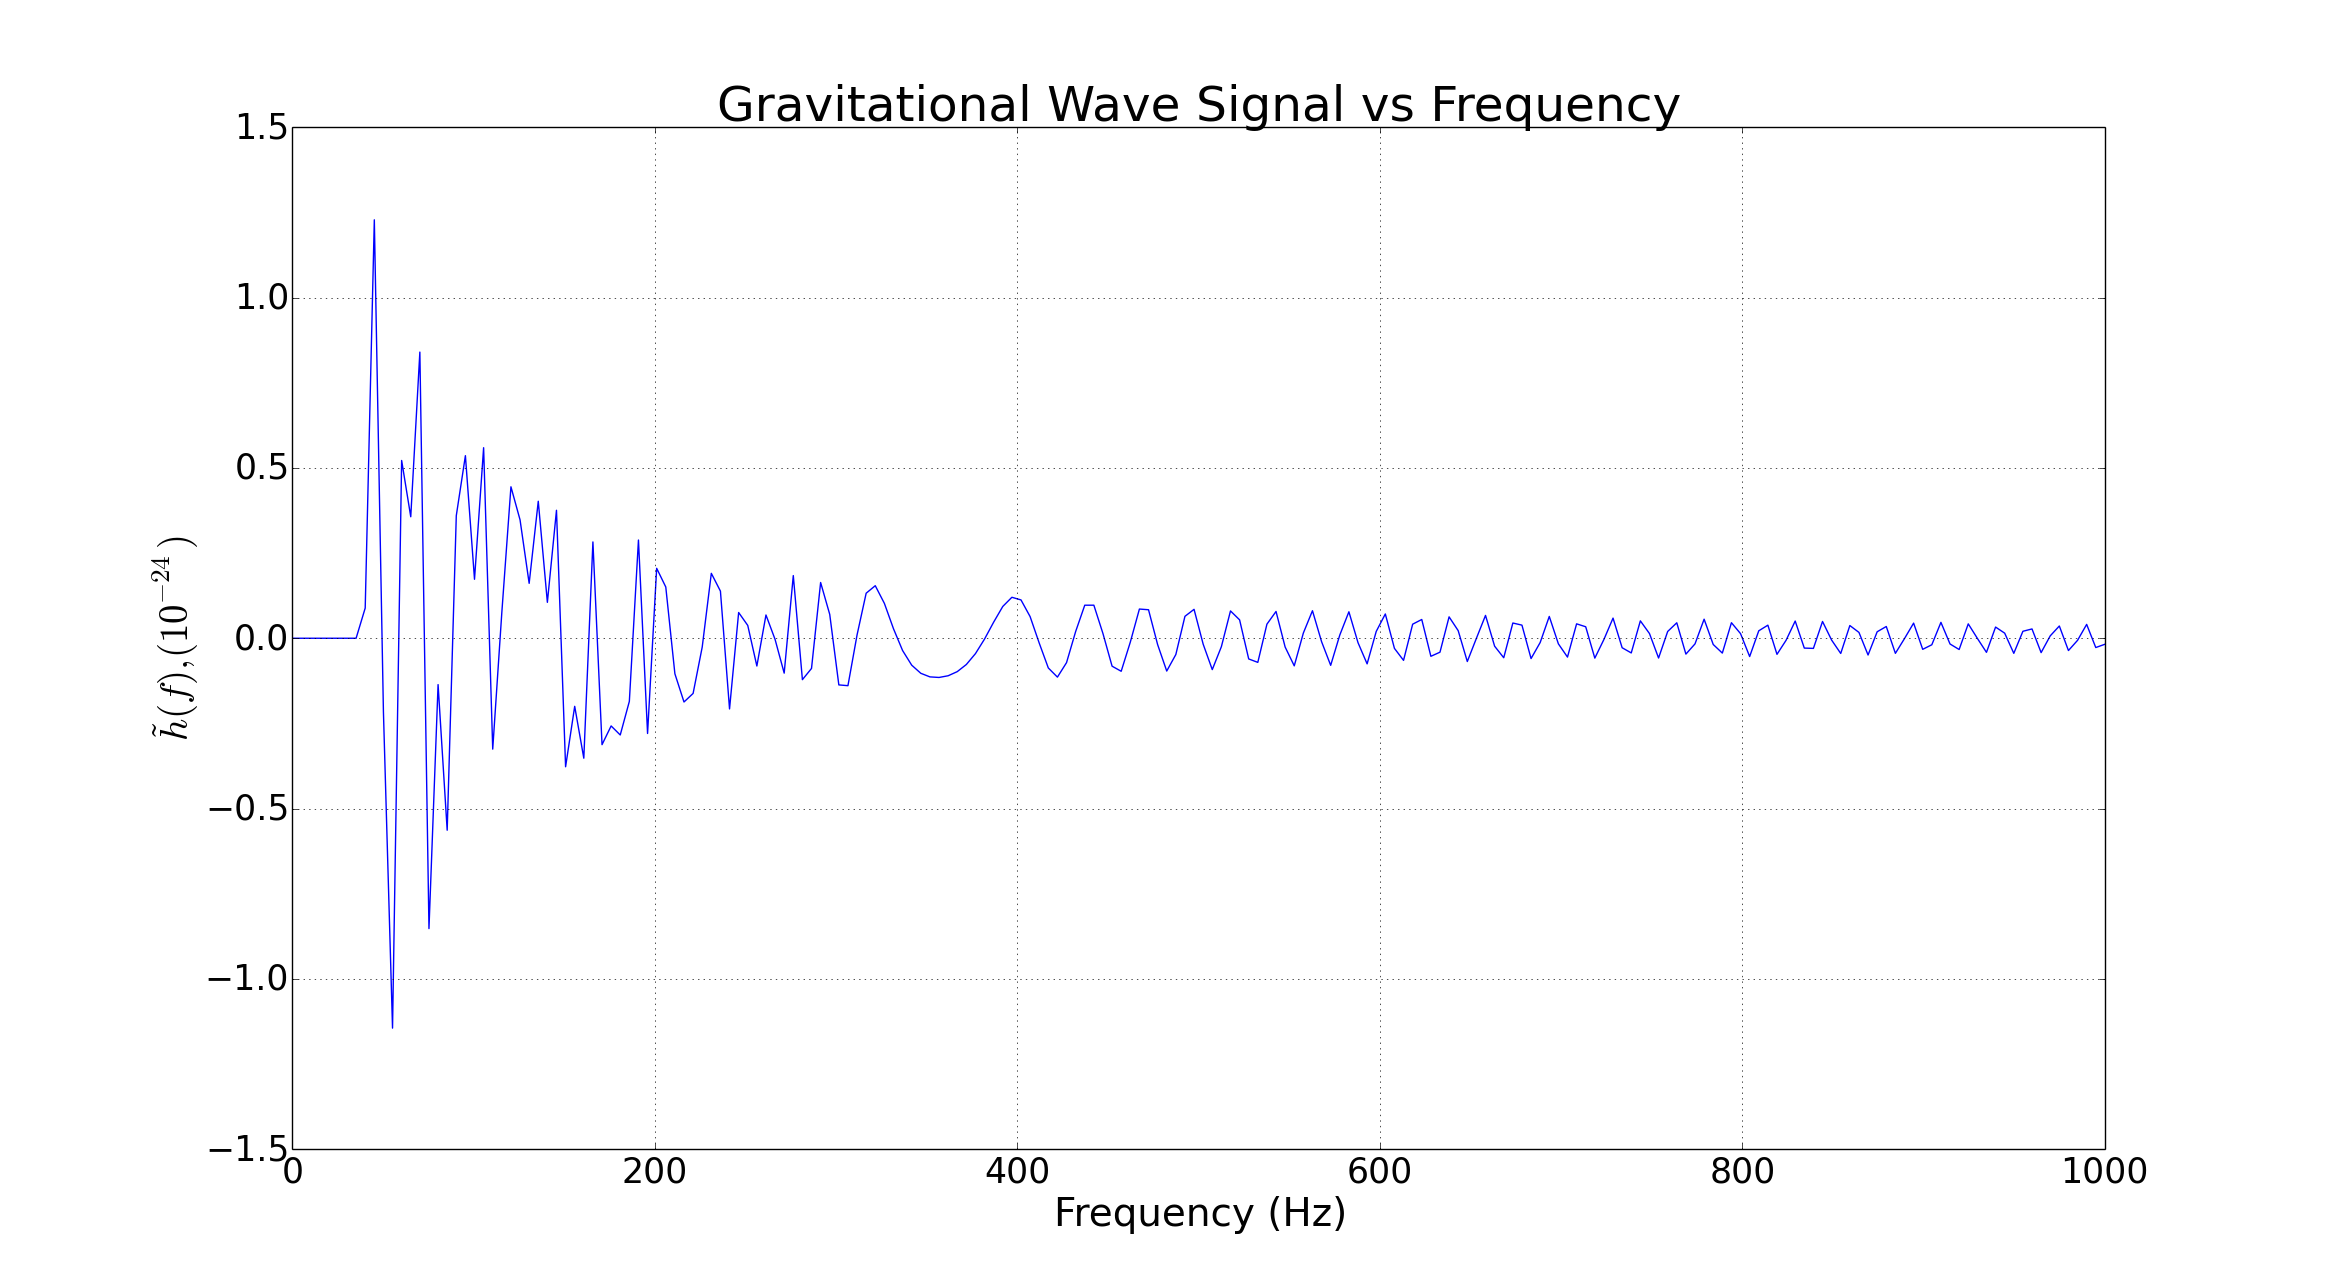
\includegraphics[width=\textwidth]{grav_signal}
  \caption{\textit{The gravitational waveform produced using coalescing binary neutron stars. The wave is represented in the frequency domain with masses $m_{1,2} = 1.4M_{\odot}$ at a luminosity distance $D_{L} = 200 \,Mpc$.}}
  \captionsetup{justification=centering}
  \label{fig:signal}
\end{figure}

%More explination
Finally, the last term in equation~\ref{eq:data} must be discussed; the noise of the model, $\tilde{n}(f)$. Throughout this project, we have added no noise to the signal, although as discussed later we do include a noise estimate in the likelihood.


%%%%%%%%%%%%%%%%%%%%%%%%%%%%%%%%%%%%

\subsection{Prior and Likelihood}
\label{sec:pandl}

The prior probability function, $p(\vec{\theta} | \curlH)$ in equation~\ref{eq:bayesgw}, represents our prior knowledge in $\theta$ before the analysis.The range of parameters used throughout this paper were chosen due to their inability to be justifiably known through a GRB assumption. The parameters were drawn from the ranges for any signals generated in this analysis, given in table 1. 

\begin{table}[H]
  \centering
  \begin{tabular}{|c|c|}
%  \caption{Prior parameters}
    \hline
    Parameter & Distribution \\
    \hline
    $\psi$   &  U($0,\pi/2$)\\
    $\iota$   & N($0,0.1$) \\
    $\phi_c$  & U($0,\pi/2$)\\
    $t_c$     & U($t_{o}-0.01, t_{o}+0.01$) \\
    $s$       & U(0,2) \\
    \hline
  \end{tabular}
  \label{tab:prior}
  \caption{\textit{The parameters used throughout the analysis with some degree of uncertainty. U(a,b) is a uniform distribution between a and b. N($\mu, \sigma$) is a normal distribution, with a mean $\mu$ and standard deviation $\sigma$. $t_{o} = 9\times10^{8}$}}
\end{table}  




Through the assumption made above allows us to constrain the system, maintaining a small number of parameters in the prior. For a realistic parameter estimation of the source, a larger range of values with a bigger distribution. This was not tested due to time constraints but is proposed as work for the future.   




The likelihood function used throughout this project is given for a generic detector D as~\cite{JVei}, 
\begin{equation}
  p(\vec{d} | \vec{\theta}, \curlH, I) \propto \exp(-(d^{D}(f) - h^{D}(f)|d^{D}(f) - h^{D}(f))/2)
\end{equation}
where $(\cdot |\cdot )$ is a representation of the inner product. This derivation is given in the appendix. Using the inner product of two real functions, and approximating for discrete integer values, the likelihood then becomes





\begin{equation}
  p(\vec{d} | \vec{\theta}, \curlH, I) \propto \exp\Bigg[ 2\Delta f\sum_{k>0}\frac{|\tilde{d}(f_{k}) - \tilde{h}(f_{k})|^{2}}{S(f_{k})} \Bigg]
\end{equation}

\begin{wrapfigure}{l}{0.5\textwidth}
  \centering
  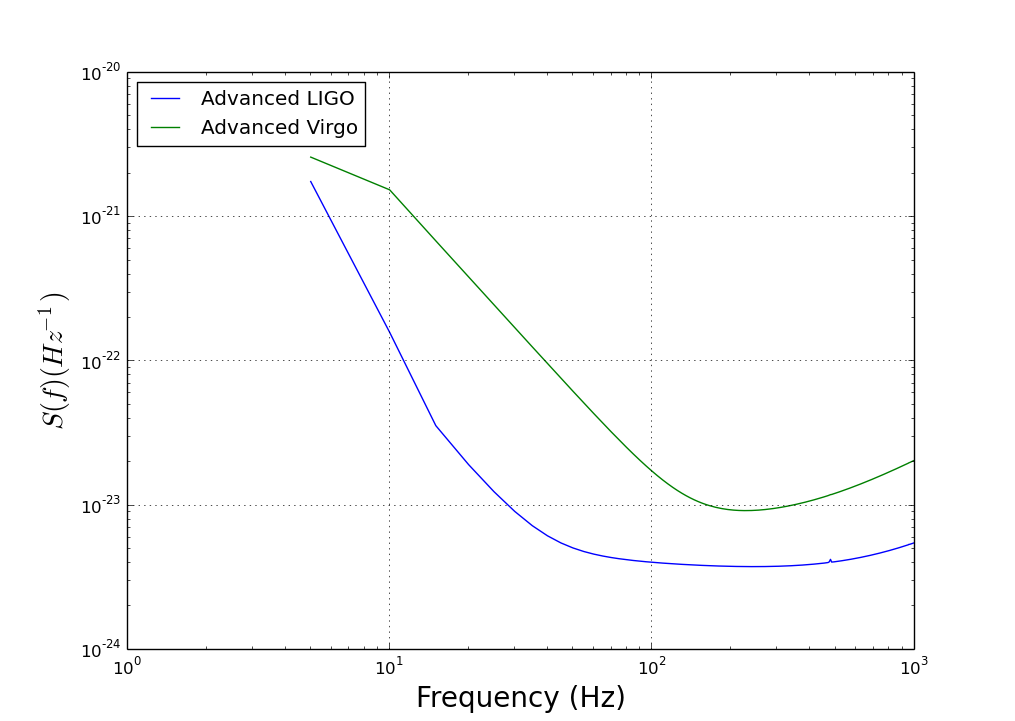
\includegraphics[width=0.5\textwidth]{PSD}
  \caption{\textit{Noise spectral density for advanced LIGO and Virgo.}}
  \label{fig:psd}
\end{wrapfigure}

where $S(f_{k})$ is the \textit{power spectral density} (PSD). This defines the sensitivity of the detector as it a measure of the strain in the detector due to noise~\cite{SathSchutz,sens}. The PSD for advanced LIGO and Virgo are shown in figure~\ref{fig:psd}. The figure shows that the strain effect for advanced LIGO is less than it is for Virgo; LIGO has a better sensitivity. This is a factor in analysing the calibration error, given in section~\ref{sec:results}. The subscript $k$ represents discrete values of relevant frequency bins (As carrying out the integral would become computationally costly). This likelihood will be used throughout the project. The factor of $\Delta f$ comes from the approximation of the inner product of two real functions (as it is integrated over frequency space).










%%%%%%%%%%%%%%%%%%%%%%%%%%%%%%%%%%%%%%%%%%%%%%%%%%%%%%%%%%%%
\subsection{Nested Sampling\label{sec:nest}}



In this paper the nested sampling method was used to solve equation~\ref{eq:bayesgw}~\cite{Sivia}. This algorithm is predominantly used in hypothesis testing, i.e. comparing a noise only data set with one possibly containing a GW to show whether there was a direct detection. As stated above, there lies a problem when solving Bayes' theorem in high dimensional parameter space. It becomes very difficult and computationally demanding when solving the integral in equation~\ref{eq:evidence}. It becomes far to complicated to compute analytically, and cannot be numerically calculated without sever computational cost.  

Nested sampling can handle this complex integral by simply changing it from a $|\vec{\Theta}|$ dimension integral into a parameter \textit{volume} integral. Equation~\ref{eq:bayesgw} becomes:

\begin{equation*}
  \Rightarrow Z = \int \limits_{\vec{\Theta}} p(\vec{d}|\vec{\theta}, \mathcal{H}) \pi \;d\pi 
\end{equation*}
\begin{equation*}
  \Rightarrow Z \approx \sum \limits_i^N p(\vec{d}| \vec{\theta_i}, \curlH) \pi_i
\end{equation*}

\begin{equation*}
  \Rightarrow Z \approx \sum \limits_i^N L_i\pi_i
\end{equation*}

where $\pi_i$ represents the \textit{prior volume} of the $i^{th}$ point in N randomly chosen positions on parameter space; N \textit{livepoints}. $L_{i}$ is the likelihood of the $i^{th}$ position. In the presence of a GW signal, the evidence is usually concentrated into one region of parameter space defined by the \textit{information} of the data set~\cite{Sivia}. It is then key to not waste computational time by analysis regions of parameter space which do not contain any information about the signal. 

N livepoints are chosen randomly in parameter space from the prior volume and $L_{i}$ and $\pi_{i}$ are calculated for each point. In this description, the prior parameters defining $\pi$ are assumed to be uniformly distributed, hence the $i^{th}$ point can be said to occupy a volume of $V_{tot}/N$ where $V_{tot}$ is the entire parameter volume.   
The process of the algorithm is carried out as~\cite{JVei}:
\begin{enumerate}
\item set $j = 0$, $Z_{j} = 0$, $\pi_{j} = 1/N$ 
\item While $Z_{j} < Z_{thresh}$:
  \begin{itemize}
  \item $j = j + 1$
  \item $L_{min} = min(\{L_{i}\})$
  \item $\pi_{j} = \pi_{j-1} - 1/N $
  \item $Z_{j} = Z_{j-1} + L_{min}\times \pi_{j}$
  \item Discard the position giving $L_{min}$
  \item Chose a new random point where $L_{new}>L_{min}$ and concatenate into $\{L_{i}\}$
  \end{itemize}

\end{enumerate}

As stated in the pseudo-code, the algorithm is dependent on a threshold term, $Z_{thresh}$. This is a value determined by the change in evidence as the algorithm is carried out. When the difference in the evidence integral between iterations becomes significantly small, then the algorithm can stop. Once the algorithm has finished the discarded livepoints can be re-sampled to give points drawn from the posterior distribution of the parameters. The accuracy of the algorithm and the parameterisation is dependent on the number of livepoints being analysed. Balancing accuracy with computational cost is one of the debated topics in GWs.





%%%%%%%%%%%%%%%%%%%%%%%%%%%%%%%%%%%%%%%%%%%%




\section{Results\label{sec:results}}

The aim of this project was to determine how well the calibration error could be parameterised in a software injected gravitational wave source. The error was estimated through numerous situations but the basis of the simulations remained the same throughout the project: a single source of GWs at varying signal to noise ratios. The GRB assumption was analysed as well by relaxing some of the defining GW paramaters and adding some uncertainty into their value, given in section~\ref{sec:pandl}. 


These values where chosen due to the assumed counterpart EM observation. These values could not be justified by that assumption so they were added into the prior with reasonable uncertainty.

The estimation of the error, given in its simplest form as a scale factor, was performed for numerous systems: single detector, a network of detectors, random sky positions, etc. Before the parameter estimation was carried out, the relationship between distance of the source relative to the detector and the signal to noise ratio (SNR) needed to be found.  

The SNR is given by
\begin{equation}
  \label{eq:snr}
  SNR = \sqrt{\Bigg( \frac{2 |\gws^D(f)|^2}{S^D(f)} df \Bigg)}
\end{equation}

where the noise spectral density, $S^D(f)$ is not a function of distance, shown in section~\ref{sec:pandl}. For coalescing binary neutron stars of masses $m_{1,2} = 1.4\,M_{\odot}$ and  $D_{L}200\,Mpc$, the expected SNR is roughly 8. The SNR was determined from $D_{L} = [10,200]\,Mpc$  using a randomly chosen sky position which defines the antenna patterns and the GW signal. The range of luminosity distance used in this paper represented a high level of SNR up to the distance at which the first predicted detectable GW source; $D_{L} = 200\,Mpc$. The detector limits for the advanced era is a luminosity distance of $\sim 450\,Mpc$. This was not initially tested as the SNR was low enough to cause problems with computational time. It was however tested in the random sky position simulations, see section~\ref{sec:rndsp}. The initial value for the calibration error used in the analysis was chosen randomly.



\begin{figure}[h]
  \centering
  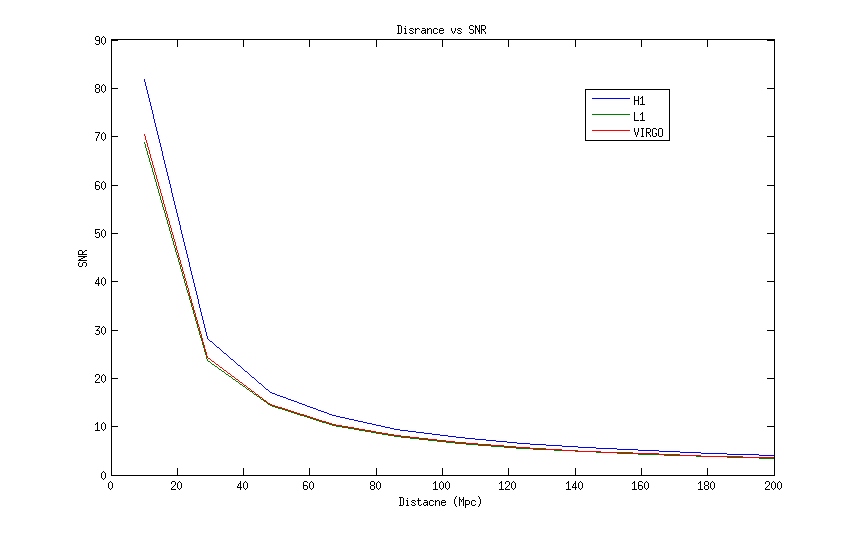
\includegraphics[width = \textwidth]{DvsSNR-mult-det}
  \captionsetup{justification=centering}
  \caption{\textit{The distance and SNR relationship for all three detectors: LIGO Hanford, H1, LIGO Livingston, L1, and VIRGO.}}
  \label{fig:distsnr}
\end{figure}



\subsection{Single Detector with GRB Observation \label{sec:sdgrb}}


To begin with, parameter estimation was carried out on the simplest case: a single source of GWs using a single detector, LIGO Hanford, at different levels of SNR. The aim was to resolve the calibration scale factor with the highest degree of certainty. 
Before testing the uncertainty resolution using a the full range of prior parameters, we fixed all values to known signal values and only searched over the scale factor. Results shown for with and without a full prior range are given in figures~\ref{fig:sd-empty-D} and~\ref{fig:sd-non-empty-D} respectively.
 

\begin{figure}[h]
  \centering
  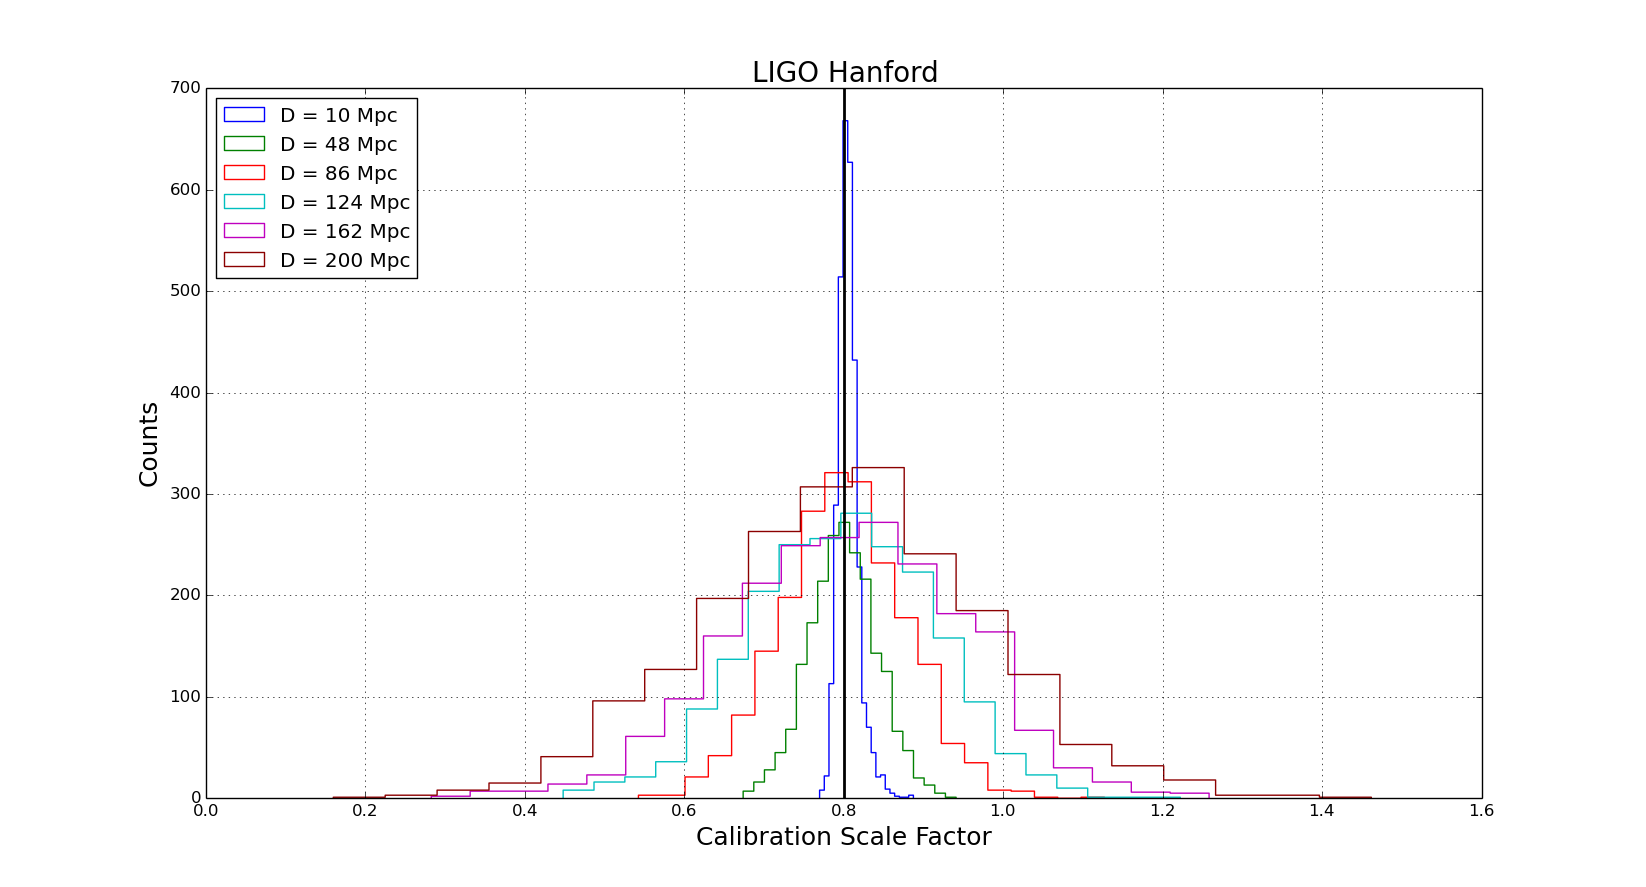
\includegraphics[width = \textwidth]{SD_empty_D10_200}
  \caption{\textit{Posterior distribution on the calibration scale factor for LIGO Hanford. Simulations carried out using an entirely known source of GWs.}}
  \label{fig:sd-empty-D}
\end{figure}

The figure above is a histogram of the calibration error, with each curve representing a different distance (SNR). The black line at $s = 0.8$ is the initial scale factor value used to multiply the unanalysed data set. This representation of the initial calibration scale factor will be continuous throughout the paper. 
One would expect with lower SNR (greater $D_{L}$), the estimation of the parameter would become less certain. This is clearly shown in figure~\ref{fig:sd-empty-D} as the standard deviations of the curves increases with smaller SNR/larger luminosity distances. For this entirely known source of GWs, we would expect to find the uncertainty in $s$ to be approximately $1/$SNR; this is what we see in figure~\ref{fig:sd-empty-D}. The error in estimating $s$ for $D_{L} = 200 \,Mpc$ is roughly $\sim 20\%$. This is larger than the current method of obtaining the uncertainty in calibration. A full test of the new method proposed is carried out in section~\ref{sec:rndsp}. 

The next estimation of the calibration scale factor was performed with a full range of prior parameters, giving a more realistic system. As before, the simulations were carried out for differing levels of SNR and a histogram of the calibration error was made, seen in figure~\ref{fig:sd-non-empty-D}.

\begin{figure}[h]
  \centering 
  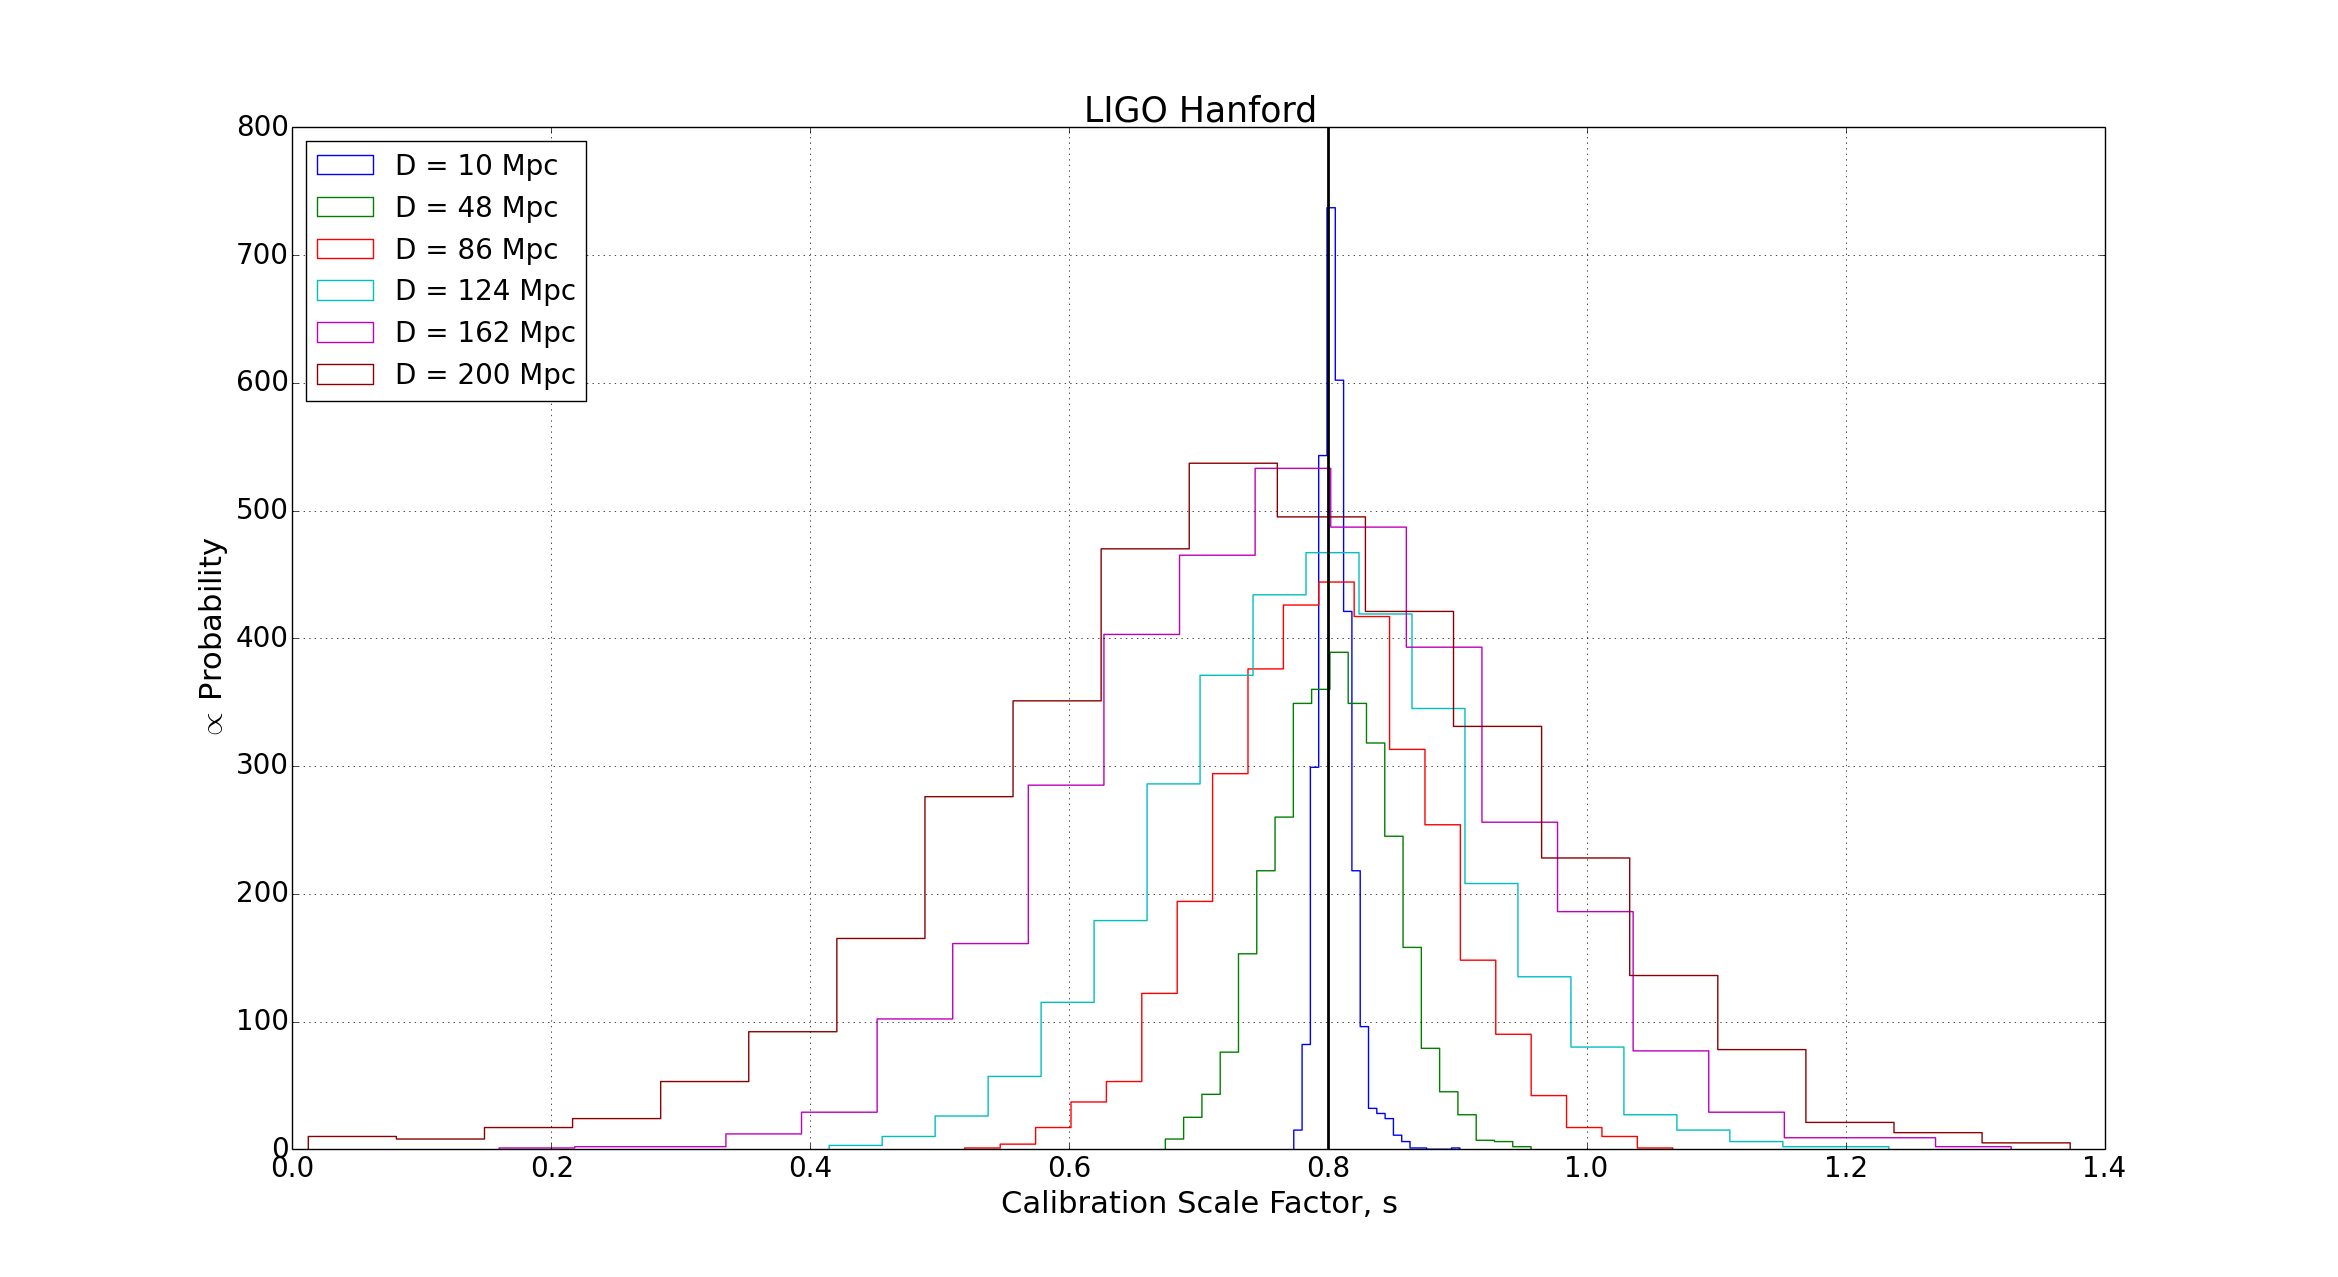
\includegraphics[width = \textwidth]{SD_non_empty_D10_200}
  \caption{\textit{Posterior distribution on the calibration scale factor for LIGO Hanford. Simulations carried out with some parameters in the prior.}}
  \label{fig:sd-non-empty-D}
\end{figure}

The error in the calibration scale factor, as before, increases with decreasing SNR (increasing $D_{L}$). The magnitude of this error however is larger than in the previous simulation. With a full prior range given in section~\ref{sec:pandl}, the standard deviation increases; at $D_{L} = 200\,Mpc$ the error in $s$ is $\sim 24\%$. When comparing this new method of calibration scale factor estimation with the current, feedback loop system method used today, this method is not as accurate. However, it should again be noted that this method is an independent estimate of the calibration accuracy.

\subsection{Multiple Detectors with GRB Observation}
\label{sec:mdgrb}
A network of detectors are used throughout GW research. Being able to show the effect of the calibration error and recovering its uncertainty in the analysis would help in giving a detection more confidence. In this section, the simulations were carried out using multiple detectors; LIGO Hanford, LIGO Livingston, and Virgo. In reality, multiple detectors are used in order to determine the (rough) sky position of a signal. Due to their locations, if one site detects a signal before the others, then the position of the source can be roughly worked out. The aim was, as before, to estimate the calibration scale factor with the least amount of uncertainty for differing levels of SNR for a single source of GWs. 

For a network of detectors, the overall likelihood function becomes a product of each likelihood for all detectors, i.e.

\begin{equation}
  \label{eq:mult-likeli}
  p(\vec{d}| \vec{\theta}, \curlH) = \prod \limits_D p(\vec{d}^D| \vec{\theta}, \curlH)
\end{equation}

where $D = \{H,L,V\}$. The initial calibration scale factors where again chosen at random ($s = [4.6, 2.5, 6.1]$ for LIGO Hanford, LIGO Livingston, and Virgo respectively). The simulations were the same as before, using the same parameter values. The GRB assumption was again tested in these simulations as a handful of parameters were relaxed and given some uncertainty. The results of these simulations are shown in figure~\ref{fig:mult-empty-D} and figure~\ref{fig:mult-non-D}.


\begin{figure}[h]
  \centering
  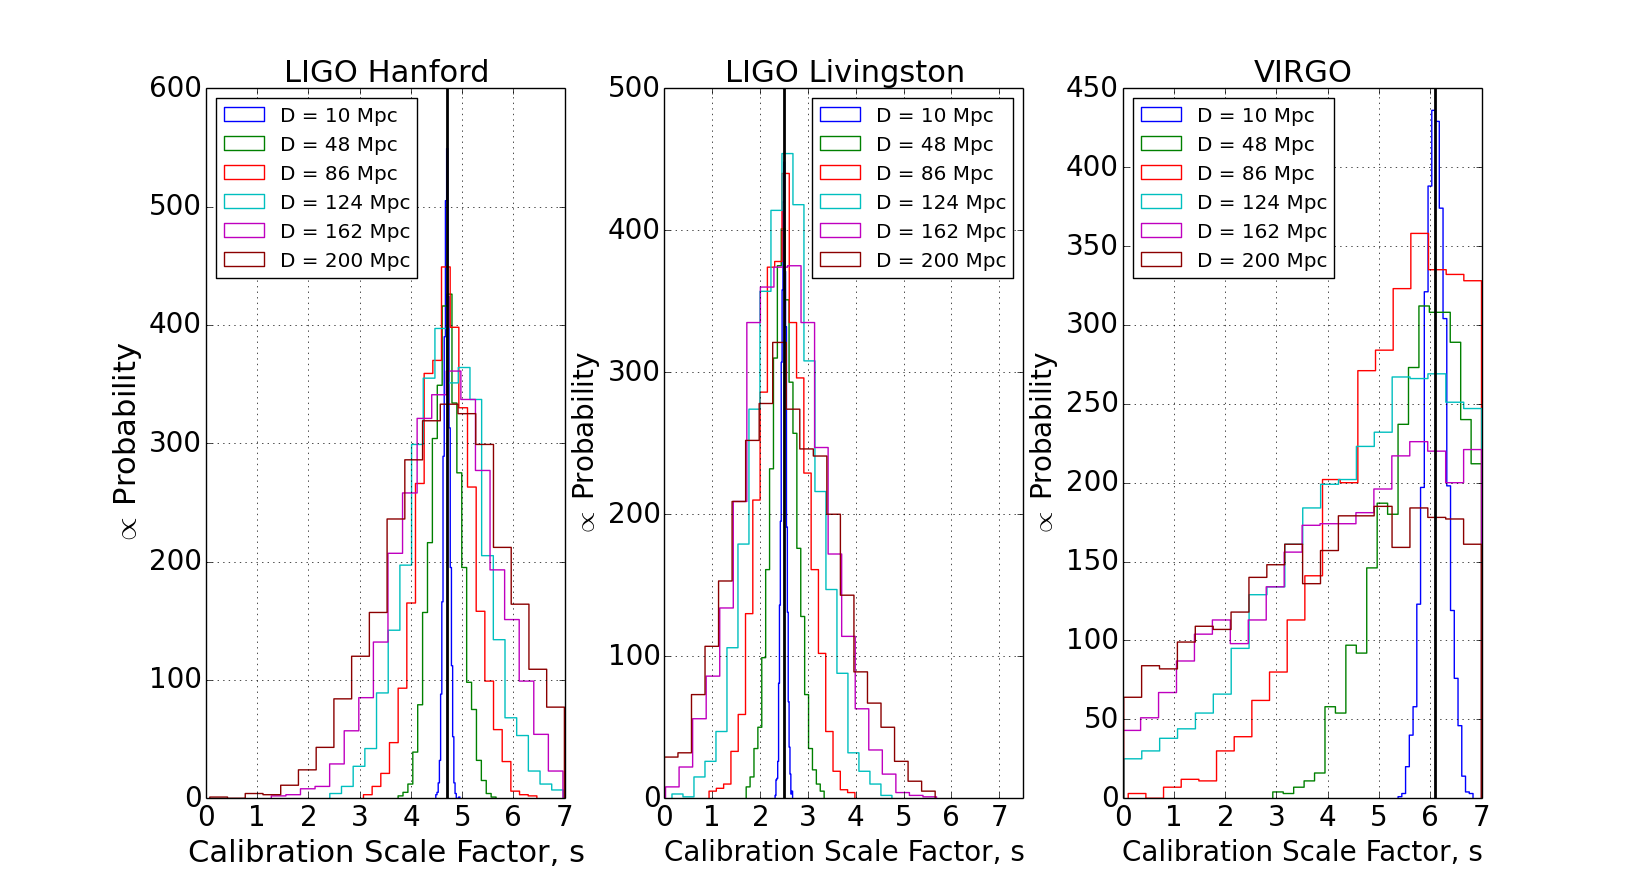
\includegraphics[width = \textwidth]{MD_empty_D10_200}
  \captionsetup{justification=centering}
  \caption{\textit{Posterior distribution on the calibration scale factor for all three detectors. Simulations carried out using an entirely known source of GWs.}}
    \label{fig:mult-empty-D}
\end{figure}

Figure~\ref{fig:mult-empty-D} shows the histograms of the calibration scale factor for each detector. These simulations used an entirely known source of GWs, at a randomly chosen sky position (the same sky position as before). As the figure shows both LIGO sites, Hanford and Livingston, are able to resolve the error with a measurable degree of uncertainty. The standard deviation for $s$ at $D_{L}=200\,Mpc$ is $24\%$ and $41\%$ of the true scale factor for Hanford and Livingston respectively. The estimation for the calibration error using VIRGO however, was not as accurate. It can be seen that, for increasing luminosity distances, the resolution of $s$ becomes increasingly uncertain until the point at which the distribution becomes almost uniform; $D_{L} \approx 120\,Mpc$. There are a few reasons why this may be. Firstly, the sky position used may not be 'ideal' for generating the antenna patterns. The most probable cause of the estimation being very poor will lie in the detector itself. The interferometer itself is not as sensitive the two LIGO sites, hence the estimation of parameters using this site will not be as precise.

\begin{figure}[h]
  \centering
  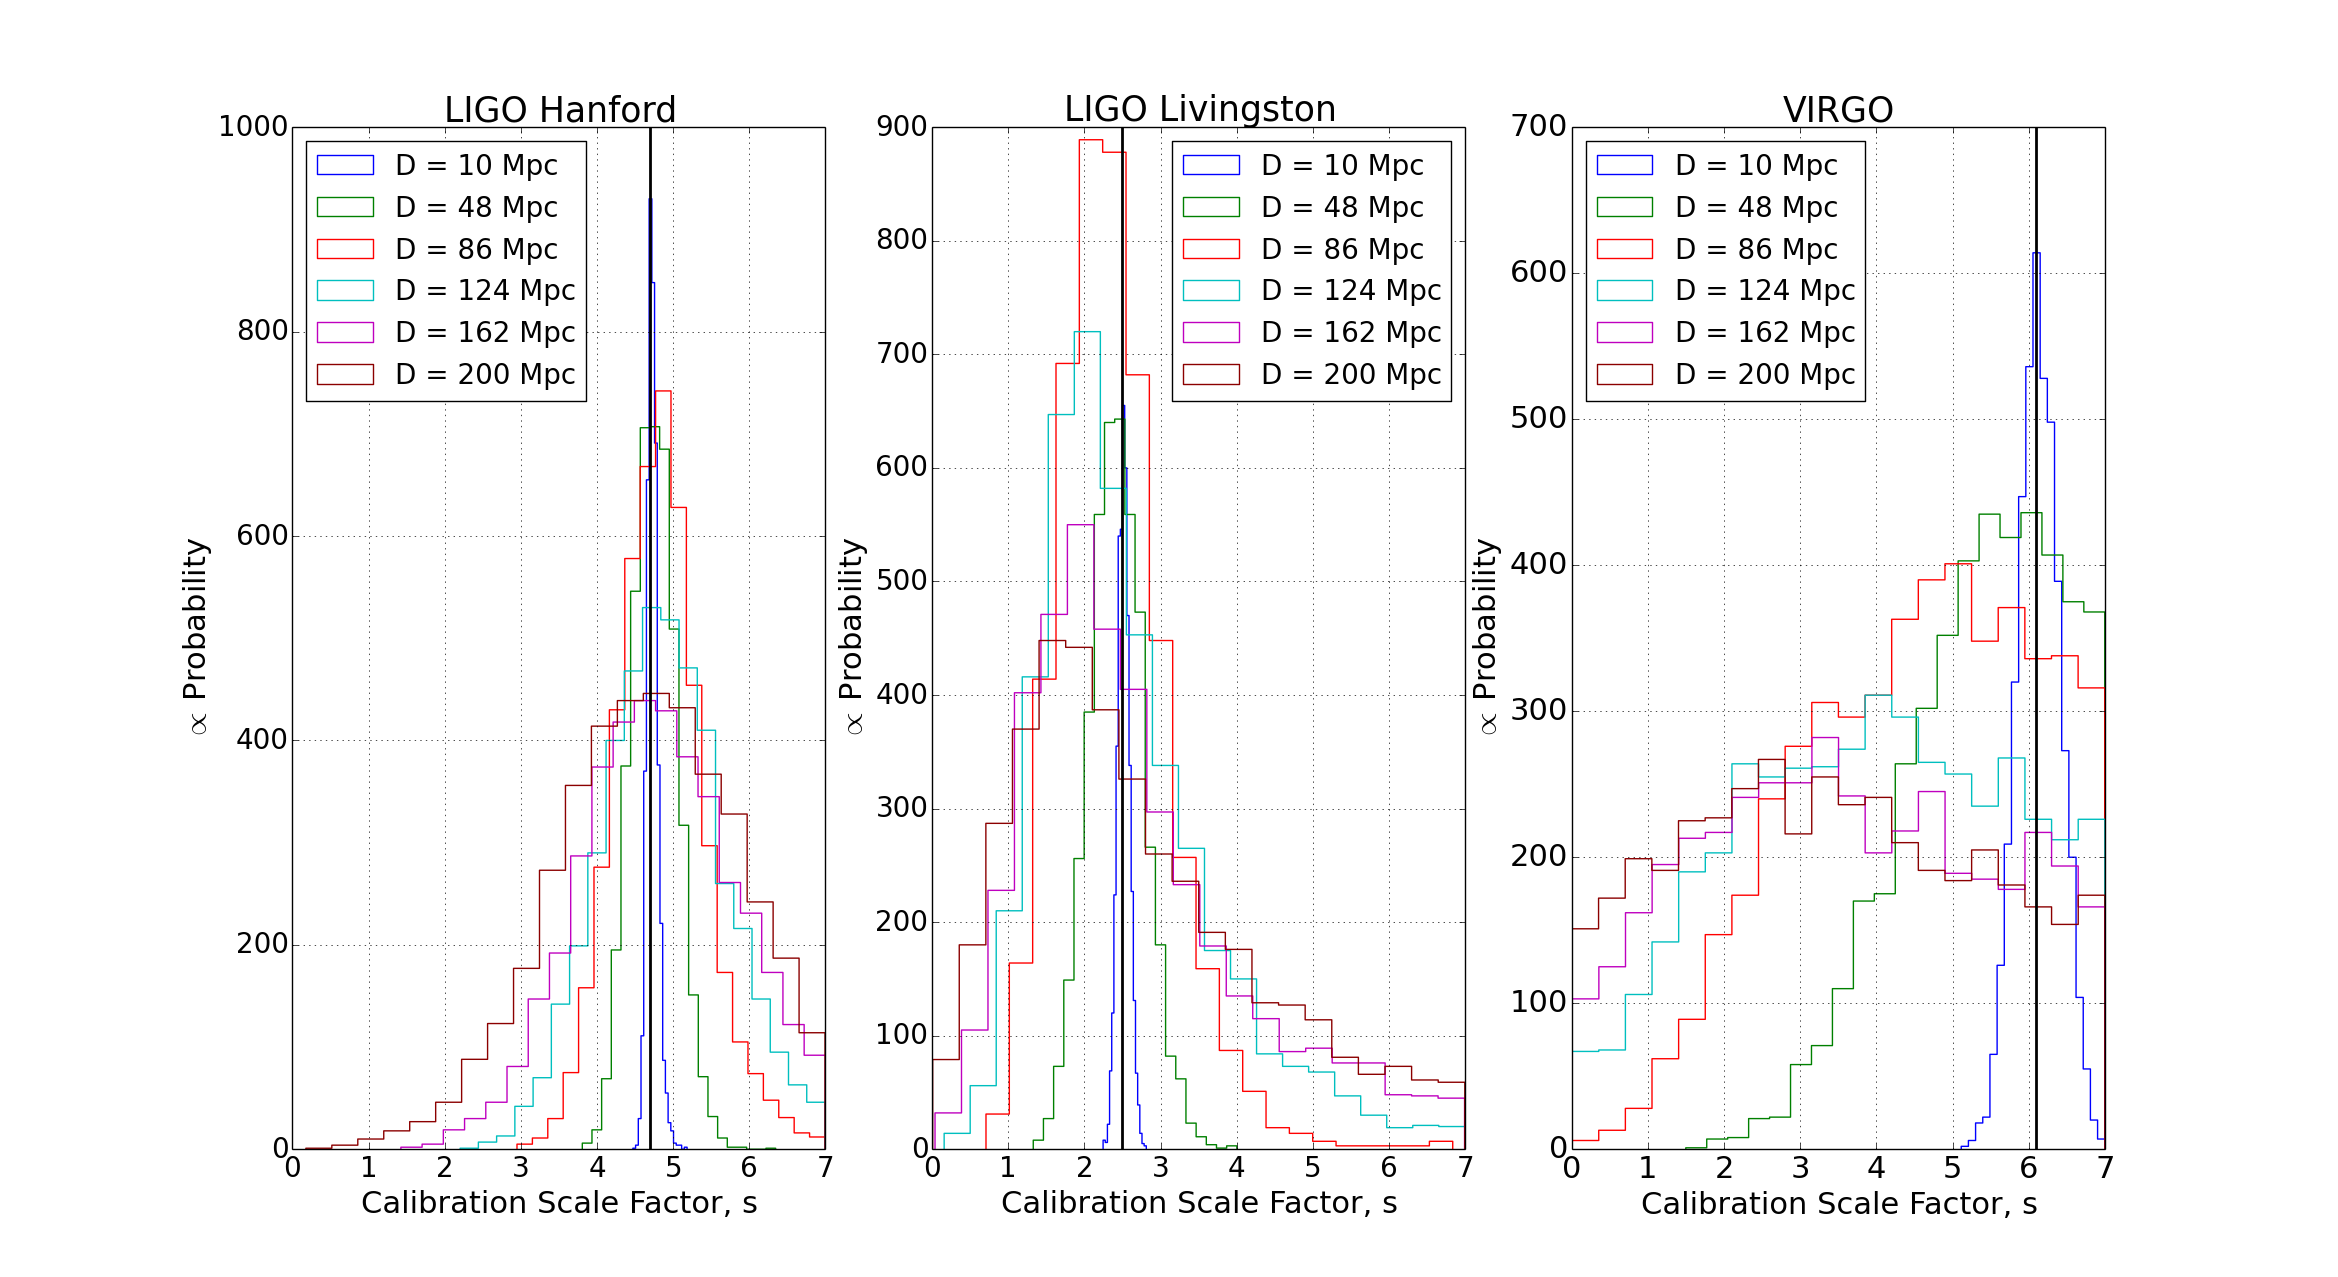
\includegraphics[width = \textwidth]{MD_non_empty_D10_200}
  \captionsetup{justification=centering}
  \caption{\textit{Posterior distribution on the calibration scale factor for all three detectors. Simulations carried out with some prior parameters. } }
  \label{fig:mult-non-D}
\end{figure}


The histograms shown in figure~\ref{fig:mult-non-D} were made using the full range of prior parameters. The uncertainty in the calibration error is larger with a less known source of GWs. VIRGO, again, has the least certain calibration error resolution with the distribution becoming even more uniform. The standard deviation for both LIGO curves become larger with increasing luminosity distance as before. For $D_{L} = 200Mpc$,  the standard deviation is $\tilde 30\%$ of the true value. When comparing this to the current method, this again is not as accurate. 

\subsection{Random Sky Position}
\label{sec:rndsp}
Throughout the duration of this project the antenna patterns were defined by a randomly chosen sky position, as seen in equation~\ref{eq:gravsig}. This did not give a true representation of the estimation capable by algorithm as this position could be a bad one; making parameterisation more difficult and less precise. To then test this new method of calibration fully, the entire field of view of the detector must be analysed. The sky positions $\alpha$, $\delta$, were distributed as:
\begin{table}[H]
\centering
  \begin{tabular}{|c|c|}
    \hline
    Parameter & Distribution \\
    \hline
    $\alpha$       & U($0$,$2\pi$) \\
    $\sin(\delta)$ & U($-1$,$1$)    \\
    \hline
  \end{tabular}
  \caption{\textit{The distribution of sky position. U(a,b) indicates a uniform distribution between a and b.}}
  \label{tab:sp}
\end{table}




Figures~\ref{fig:snr-rndsp} and~\ref{fig:std-rndsp} were obtained using a luminosity distance $D_{L} = 200 Mpc$ as this is the expected luminosity distance predicted to host the first observable GW~\cite{peadvanced}. $100$ different sky positions were tested using the LIGO Hanford site. The number of locations was limited by the length of time these simulations took to carry out. Increasing the number of locations would give a more accurate representation of the estimation ability; this can be carried out in future. Finally, a full range of prior parameters were also used in the simulation set-up. 



\begin{figure}[h]
  \centering
  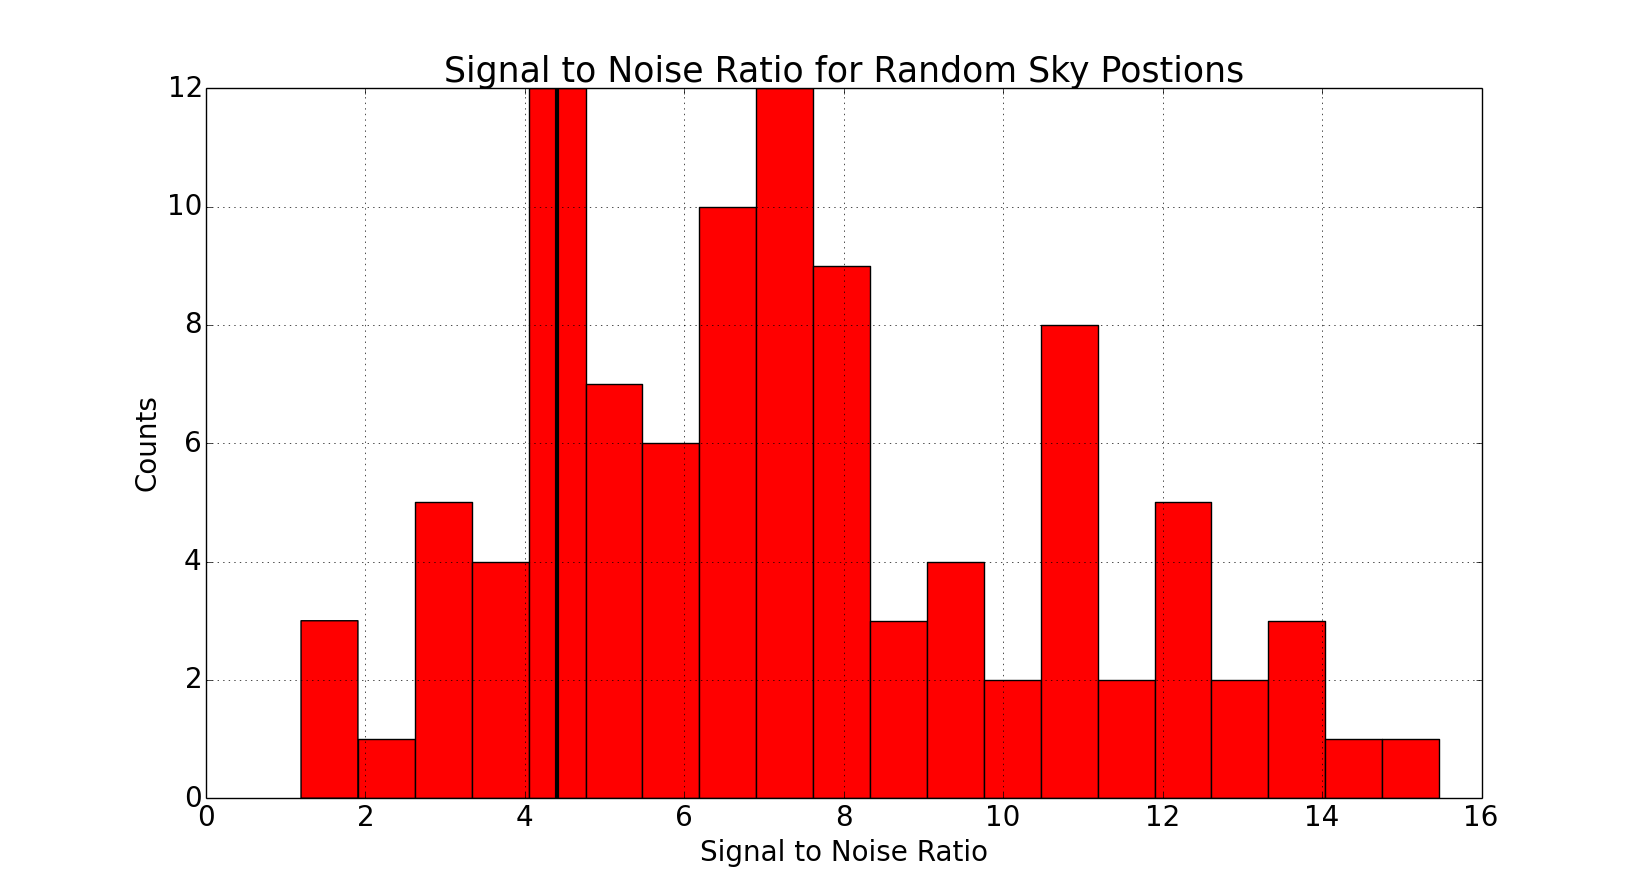
\includegraphics[width=\textwidth]{rand_sp_snr_D200}
  \caption{\textit{Signal to noise ratio for every sky position analysed at $D_{L} = 200 \,Mpc$. The vertical black line represents the SNR for the sky position used throughout previous simulations}}
  \label{fig:snr-rndsp}
\end{figure}







Figure~\ref{fig:snr-rndsp} shows the histogram of SNRs for the entire field of view for the detector. Predictions state that at a luminosity distance of $D_{L}=200\,Mpc$, the SNR will be roughly 8. This is consistent with the results obtained. The vertical black line shown in figure~\ref{fig:snr-rndsp} represents the SNR used throughout the project using the randomly chosen $\alpha$ and $\delta$. One can see that this is a less-than-average SNR and may explain the resolution of the calibration error not being too precise. This then is a promising result and the full testing of this new calibration method can be carried out. 


\begin{figure}[h]
  \centering
  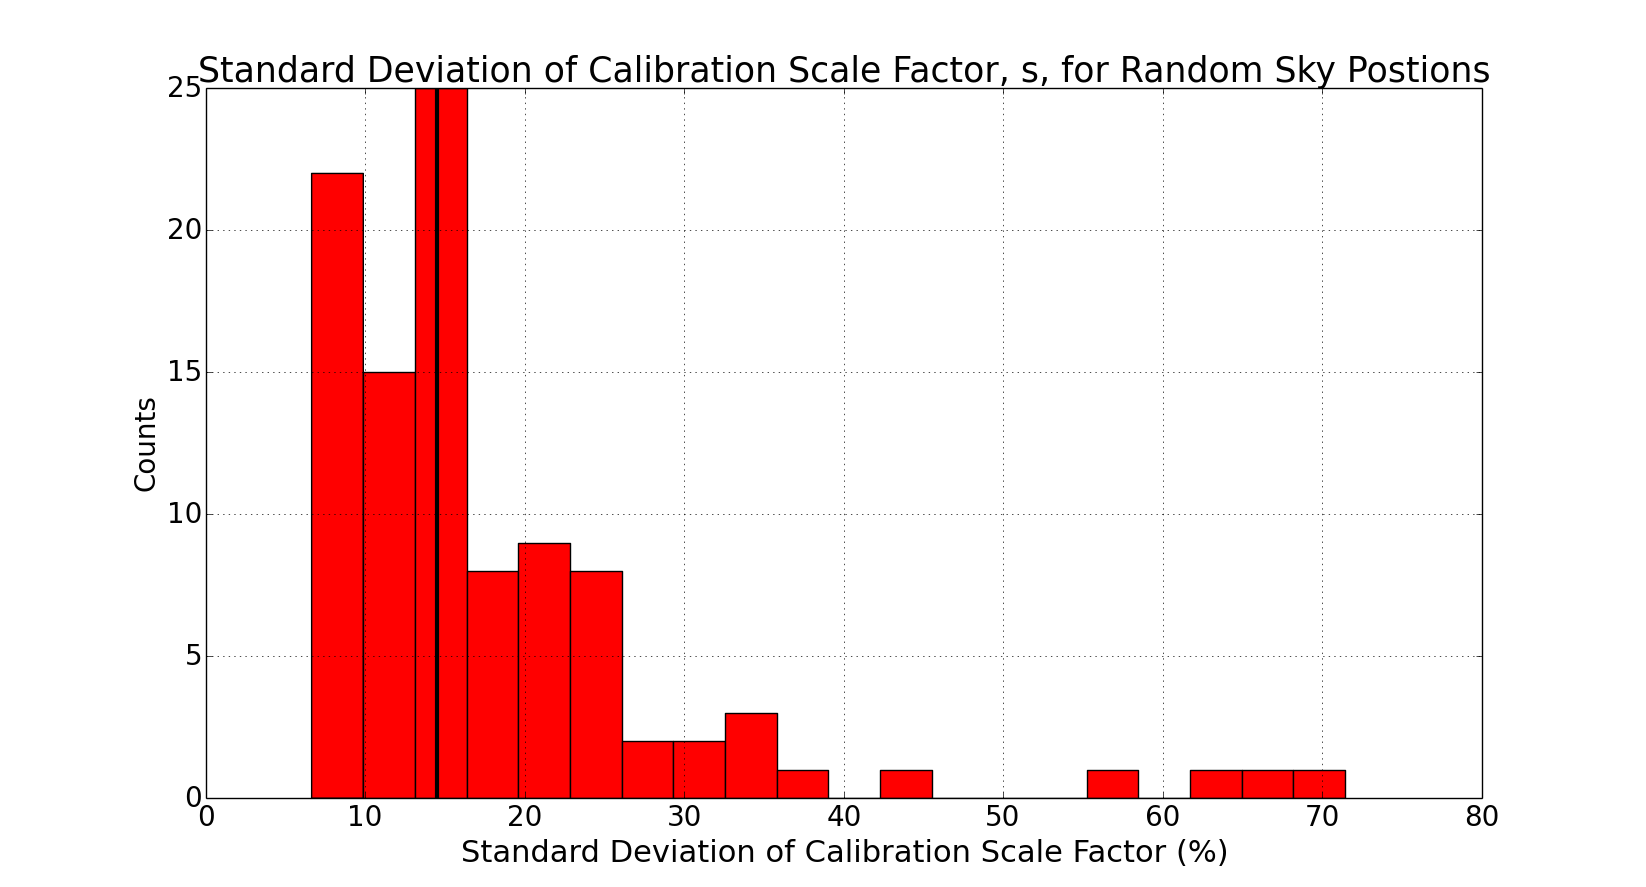
\includegraphics[width=\textwidth]{rand_sp_std_D200}
  \caption{\textit{Standard Deviation (as a $\%$ of the true scale factor value) for every sky position analysed at $D_{L}=\,200Mpc$. The vertical black line indicates the median of the distribution.}}
  \label{fig:std-rndsp}
\end{figure}



Figure~\ref{fig:std-rndsp} is the distribution of fractional standard deviations on s for each sky position analysed, given as a percentage. The vertical black line in this figure shows the \textit{median} of the distribution. The results show that the algorithm can resolve the calibration error in the data within the range of $\sim 7\%$ to $\sim 14\%$ of the true value of $s$, for $D_{L}=200\,Mpc$. Being able to recover the scale factor error to this accuracy range confirms that the new method of calibration method is very competative with current techniques. These results also confirm that the sky position used throughout the project was indeed a bad choice with an error estimation of $\sim 24\%$.


Other simulations relating to the randomisation of $\alpha$ and $\delta$ were carried out in this project. Different luminosity distances were simulated to test different levels of SNR. The expected trend was that the standard deviation scales with SNR; with high SNR yielding a better resolution of the scale factor error. The results show this trend, given in table 

\begin{table}[H]
  \centering
  \begin{tabular}{|c|c|c|}
    \hline
    Distance ($Mpc$) &$\langle$ SNR $\rangle$ & median(Standard Deviation)($\%$) \\
    \hline 
    $20$ & 74 & 1.5 \\
    $120$ & 12  & 7 \\
    $450$ & 3 & 27\\
    \hline
  \end{tabular}
  \caption{\textit{Random sky positions for different luminosity distances; $\langle$SNR$\rangle$ is the mean SNR for the distribution. }}
  \label{tab:dist-randsp}
\end{table}

The last, and lengthiest, set of simulations carried out used a network of detectors. Analysis on a luminosity distance of $200 \,Mpc$ was the only one carried out in this paper. This was due to time taken to process these simulations. With a full prior range and $100$ random sky positions as before, the standard deviations and SNRs were obtained. Results are shown in~\ref{tab:mult-rndsp}.


\begin{table}[H]
\centering
\begin{tabular}[H]{|c|c|c|}
\hline
  Detector   & $\langle$SNR$\rangle$ & median(Standard Deviation)($\%$)\\
\hline
LIGO Hanford & 20& 3 \\
LIGO Livingston & 20 & 10 \\
Virgo & 5 & 30\\
\hline
\end{tabular}
\caption{\textit{Results from randomising the sky position using a network of detectors with a full range of prior parameters at $D_{L} = 200\, Mpc$.}}
\label{tab:mult-rndsp}
\end{table}


Table~\ref{tab:mult-rndsp} gives promising results for both LIGO sites. One can see that the error estimation for LIGO Hanford is very good, with half of the positions analysed having an uncertainty $<3\%$. One would expect the gap in estimation accuracy between the two LIGO sites to be smaller as they are built to the same sensitivity. This leads to the conclusion that not enough sky positions were analysed. Virgo again has a less accurate recovery of the calibration scale factor. As mentioned above, the larger uncertainty is expected to originate from the sensitivity of the detector itself.  

\section{Conclusion \& Discussion}
\label{sec:concl}

This paper has shown that for differing levels of SNR, the error in the calibration is resolved within a certain accuracy range. Initial simulations used a bad sky position, resulting a low SNR which created larger uncertainty in resolving $s$. It was shown that for this sky position, the calibration scale factor estimation was recovered with an accuracy of roughly a $27\%$ for $D_{L} = 200\,Mpc$ for LIGO Hanford. The resolution of $s$ for a network of detectors was also shown.  

The main results obtained in this project were from analysing randomly chosen sky positions from the entire field of view for the detector. Through these simulations, it was shown that this new method of calibration can reach and surpass the current method in terms of accuracy. The results in figure~\ref{fig:std-rndsp} show that for half of the randomly chosen sky positions relate to an estimation of $s$ within a range comparable with the current methods. 

These results are reassuring for parameter estimation of the defining GW signal and would help in reducing the uncertainty in a direct detection. This project was; however, time constrained. There are many, many things that could be done with this project. A true noise realisation with each frequency bin having a random Gaussian noise would be the next step in calibration error estimation.

This project is only the beginning in testing this new method of calibration. More rigorous testing has to be carried out for a number of different systems. As mentioned above, a larger number of random sky positions have to be analysed to give better understanding of the resolution capabilities of the method. The current technique of calibration defines the error in the detector to be a complex function of frequency and phase of the GW. Instead of the simple scale factor used so far, a more realistic error can be tested to ensure that the estimation in its value is still comparable with current methods. 


For applications of this calibration method, hypothesis testing could be carried out. Testing different hypothesis is the technique used in determining a GW signal in a data-set when compared to a noise-only data-set. Being able to show with confidence that the data contains a signal is the primary focus of GW research at the moment. Therefore if uncertainty can be removed from the analysis this will ensure a more confident detection. Using this new method is resolving and removing the uncertainty is an area which has to be explored.
 

\section{Acknowledgements}
\label{sec:ackn}

I would like to thank my supervisors, Dr. Matthew Pitkin and Dr Christopher Messenger, for their help and guidance throughout the project. Without their help, bug fixing in code would have been an arduous task.



\section*{Appendix}
The inner production of two real functions, $a$ and $b$, is given as
\begin{equation}
  (a|b) = 2 \int_0^{\infty} \frac{a(f)b^*(f) + a^*(f)b(f)}{S(f)} \, df
\end{equation}
\begin{equation}
  \label{eq:blah}
  \approx 2 \Delta f \sum_{k>0} \frac{a(f_{k})b^*(f_{k}) + a^*(f_{k})b(f_{k})}{S(f_{k})}
\end{equation}
 where the integral has been approximated to a summation over discrete frequency bins, $f_{k}$. When the inner product of one real function $a(f)$, 15 becomes
 \begin{equation}
   (a|a) = 2 \Delta f \sum_{k>0} \frac{|a(f_k)|^{2}}{S(f_{k})}
 \end{equation}

For the likelihood considered in this project,
 \begin{equation}
    p(\vec{d} | \vec{\theta}, \curlH, I) \propto \exp\Bigg[ 2\Delta f\sum_{k>0}\frac{|\tilde{d}(f_{k}) - \tilde{h}(f_{k})|^{2}}{S(f_{k})} \Bigg]
 \end{equation}


\section{References}
\label{sec:ref}

\bibliography{references}





\end{document} 